\section{Flusso in un condotto piano}
La presente indagine si pone come obiettivo quello di valutare l'andamento del coefficiente di caduta di pressione $\lambda$ al variare del numero di Reynolds in un condotto piano. Pertanto, si procede con la misura della distribuzione di pressione statica lungo il condotto al variare della portata ovvero del numero di Reynolds. Quindi si valuta il gradiente di pressione $dp/dx$ per ogni portata e successivamente si calcola il coefficiente di caduta di pressione per ogni numero di Reynolds.\\\\
I dati sperimentali $\lambda=\lambda(Re)$ vanno confrontati con gli andamenti delle leggi canoniche valide per il flusso in un condotto. Dallo studio dovrà emergere il valore del numero di Reynolds critico per il condotto in esame.
\begin{figure}[H]
    \centering
    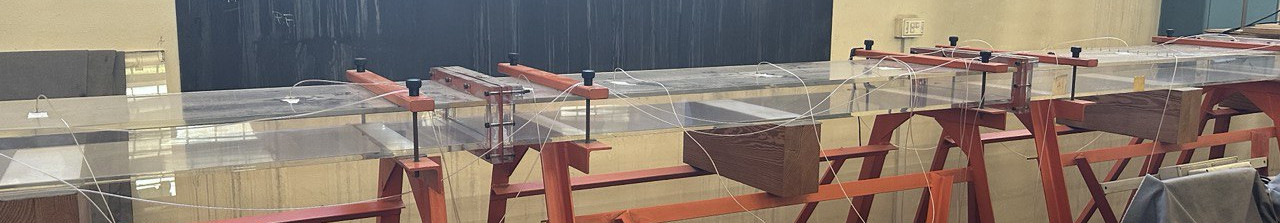
\includegraphics[width=\textwidth]{images/7/condotto.jpg}
    \caption{Condotto piano a sezione rettangolare in esame}
\end{figure}

\subsection{Descrizione dell'esperimento}
Per un generico flusso in un condotto piano, all'entrata di tale condotto si generano due strati limite. Dopo una certa distanza dall'entrata, detta lunghezza di imbocco, gli strati limite interferiscono tra loro e generano un profilo di velocità che si mantiene costante lungo il condotto, con la massima velocità in corrispondenza dell'asse. Si parla quindi di flusso completamente sviluppato.
\begin{figure}[h]
    \centering
    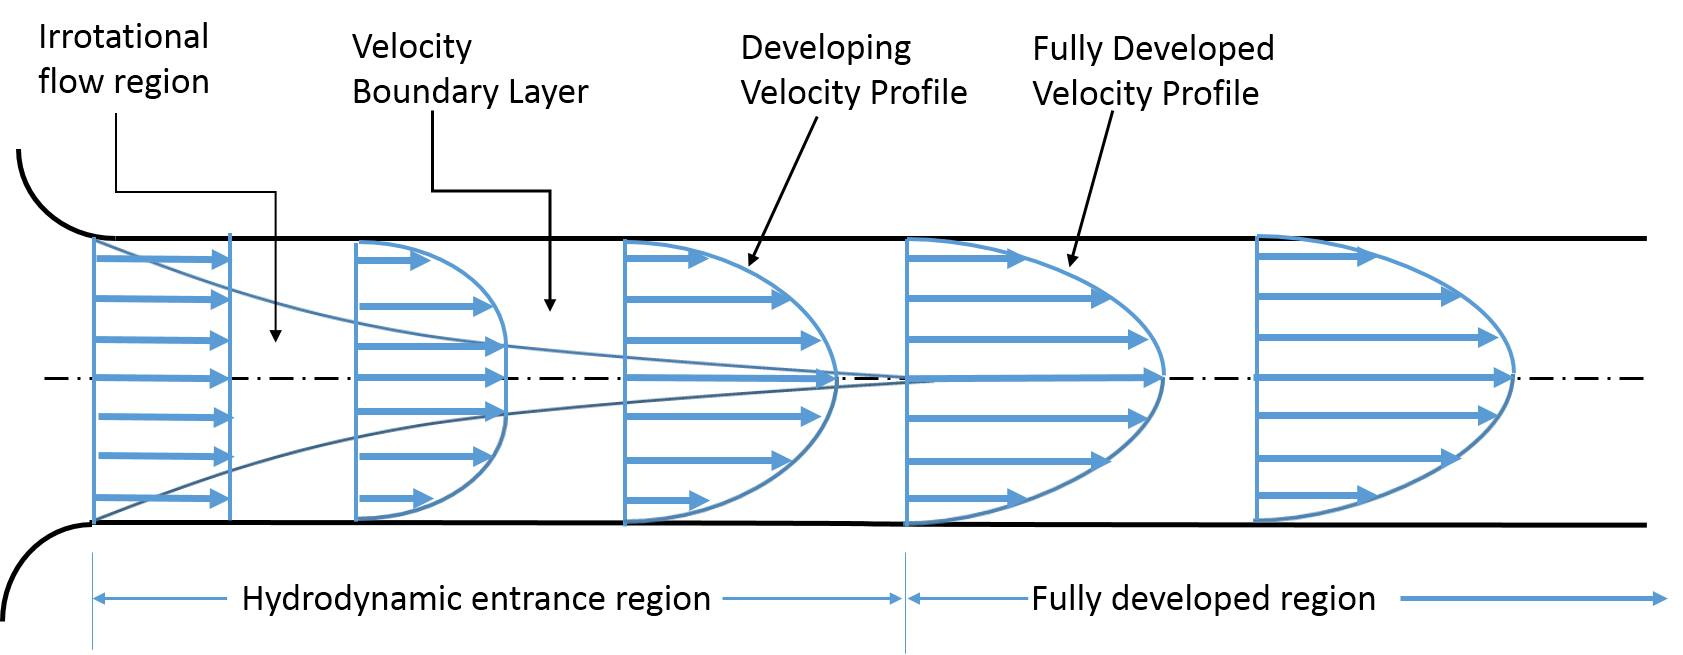
\includegraphics[width=\textwidth]{images/7/fullydeveloped.jpg}
\end{figure}

\noindent Poiché i profili di velocità nel condotto sono costanti, allora anche la velocità rimane costante, pertanto si parla di flusso congelato:
\begin{equation*}
    \frac{\partial u}{\partial x} = 0
\end{equation*}
Nel caso di una galleria del vento, il flusso in camera di prova si può considerare da subito già completamente sviluppato. Poiché il flusso risulta quindi congelato, allora le forze d'inerzia sono nulle, quindi la pressione dinamica rimane costante lungo $x$.\\\\
Poiché sulla parete del condotto si sviluppano effetti viscosi, la pressione totale diminuisce e risulta che la pressione statica decade linearmente lungo il condotto. Pertanto il gradiente di pressione $dp/dx$ rappresenta un valore costante e negativo.\\\\
Il coefficiente di caduta di pressione $\lambda$ è un parametro adimensionale che caratterizza il gradiente di pressione in un condotto, è quindi definito come:
\begin{equation*}
    \lambda = \frac{dp/dx}{\frac12 \rho \overline U^2 / D_{idr}}
\end{equation*}
Dove $D_{idr}$ è il diametro idraulico, ovvero il diametro equivalente che una sezione generica avrebbe se fosse circolare. Per una sezione rettangolare, di base $B$ ed altezza $H$, il diametro idraulico si calcola come:
\begin{equation*}
    D_{idr} = \frac{4A}{P} = \frac{4BH}{2(B+H)}
\end{equation*}
Per un generico volume di controllo di lunghezza $\Delta x$ in un condotto piano a sezione rettangolare, tale per cui $B>>H$, si può scrivere il seguente bilancio di forze:
\begin{equation*}
    p(HB) - (p+\Delta p)(HB) - 2\tau_w (B\Delta x) = 0
\end{equation*}
Dove $p$ è la pressione applicata in corrispondenza della superficie del volume di controllo alla coordinata $x_0$ e $p+\Delta p$ è la pressione applicata in corrispondenza della superficie del volume di controllo alla coordinata $x_0+\Delta x$ ($\Delta p$ è quindi un valore negativo). Poiché $B>>H$, si possono trascurare le forze viscose agenti sui due lati più piccoli.\\\\
Dal bilancio di forze si ricavano quindi gli sforzi di attrito a parete $\tau_w$:
\begin{equation*}
    \tau_w = -\frac{\Delta p}{\Delta x} \frac H2 = \left| \frac{\Delta p}{\Delta x} \right| \frac H2
\end{equation*}
Risulta quindi che gli sforzi di attrito a parete in un condotto piano dipendono solo dall'entità del gradiente di pressione e dall'altezza del condotto.

\newpage
\subsection{Catena di misura}
Il condotto a sezione rettangolare in esame ha lunghezza $L=10$ m, spessore $B=0.3$ m e altezza $H=0.07$ m. A monte della camera di prova è presente il convergente ed una camera di tranquillizzazione, per stabilizzare il flusso ed abbattere la turbolenza.
\begin{figure}[H]
    \centering
    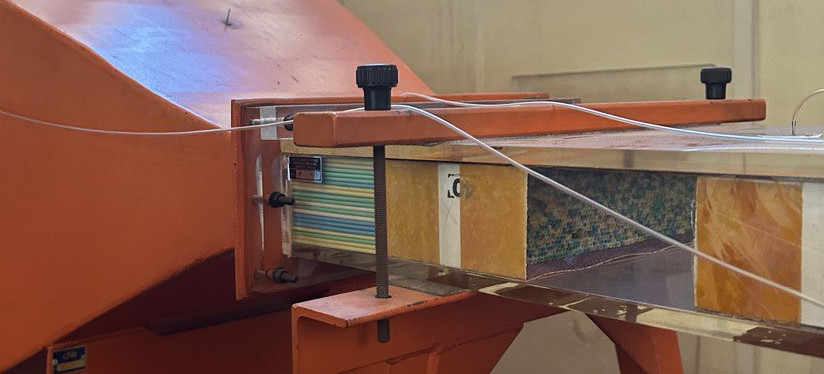
\includegraphics[width=.9\textwidth]{images/7/cannuccie.jpg}
    \caption{Honeycomb artigianale per stabilizzare il flusso}
\end{figure}

\noindent Il numero di giri della ventola, e quindi la portata del flusso, è regolato tramite un semplice pannello di controllo.
\begin{figure}[H]
    \centering
    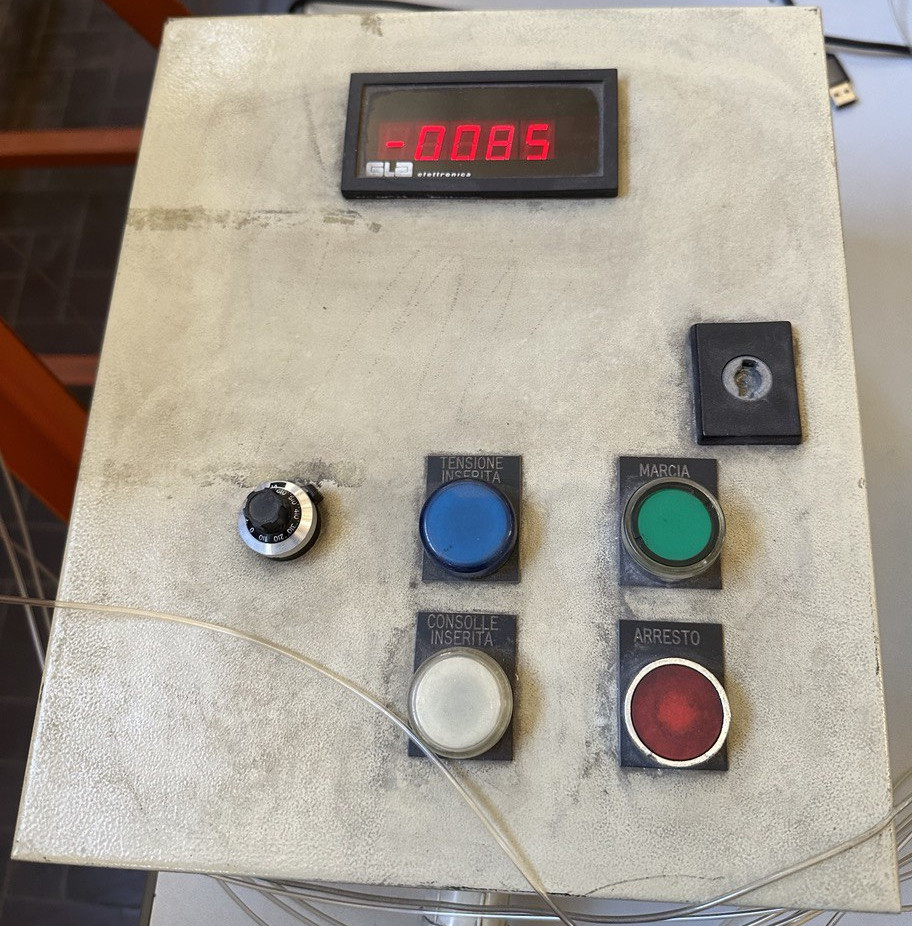
\includegraphics[width=.45\textwidth]{images/7/regolatoreportata.jpg}
    \caption{Pannello di controllo per la regolazione della portata}
\end{figure}

\noindent Lungo il condotto sono presenti 11 prese di pressione statica, posizionate sulla parete superiore in corrispondenza della mezzeria del condotto.\\\\
Le prese di pressione statica sono posizionate alle seguenti coordinate:
\begin{equation*}
    x = [0,\ 0.38,\ 0.76,\ 1.185,\ 1.401,\ 1.785,\ 2.17,\ 2.59,\ 2.82,\ 3.19,\ 3.8]\ \text{m}
\end{equation*}
In aggiunta alle 11 prese di pressione statica, sono presenti due altre prese di pressione, una per la pressione totale ed una per la pressione statica, affinché si possa misurare la pressione dinamica e quindi la velocità del flusso sull'asse del condotto.
\begin{figure}[H]
    \centering
    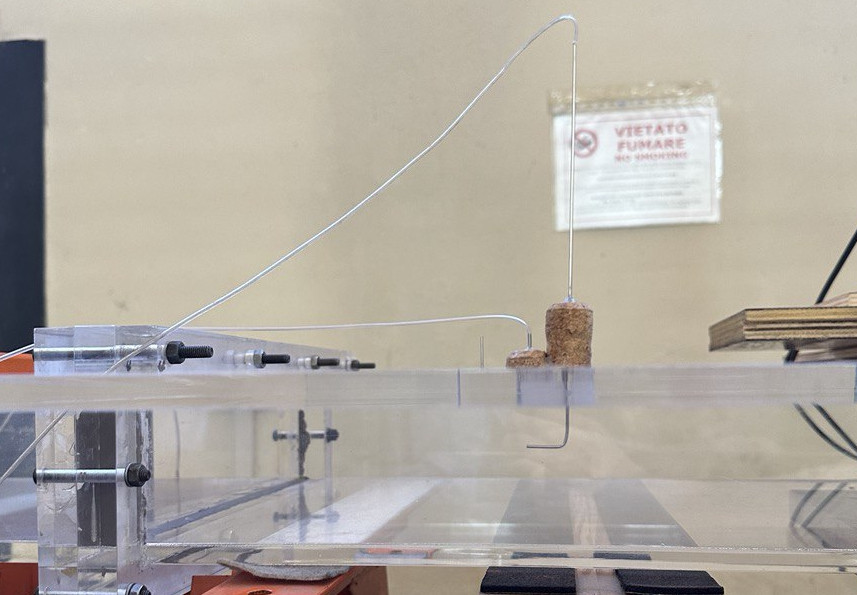
\includegraphics[width=.55\textwidth]{images/7/prese.jpg}
    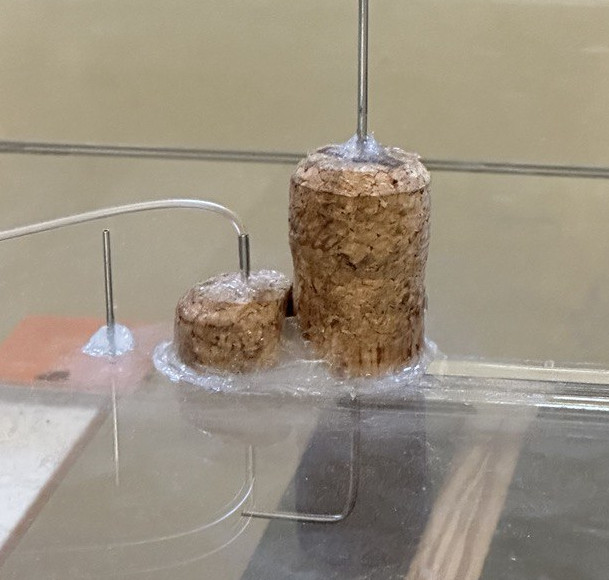
\includegraphics[width=.401\textwidth]{images/7/sughero.jpg}
    \caption{Prese di pressione statica e totale nel condotto}
\end{figure}

\noindent Le complessive 13 prese di pressione sono connesse mediante dei condotto pneumatici ad un trasduttore di pressione differenziale piezoresistivo, il DSA 3217.
\begin{figure}[H]
    \centering
    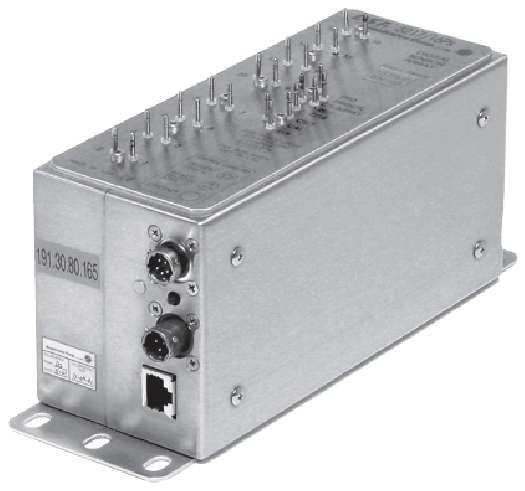
\includegraphics[width=.35\textwidth]{images/7/trasduttore.png}
    \caption{Trasduttore di pressione DSA3217}
\end{figure}

\noindent Questo trasduttore permette di acquisire ben 16 canali di pressione differenti. Nell'indagine in esame sono necessari solo 13 canali, pertanto le ultime 3 prese di pressione sono scollegate. Anche la presa dedicata alla pressione di riferimento è lasciata scollegata, in questo modo la pressione di riferimento coincide con la pressione ambiente.
\newpage
\noindent In particolare, il primo canale corrisponde alla presa di pressione totale, il secondo alla presa di pressione statica in corrispondenza della presa di pressione totale, mentre i canali dal terzo al tredicesimo rilevano le pressioni statiche lungo la direzione $x$ del condotto.
\begin{figure}[H]
    \centering
    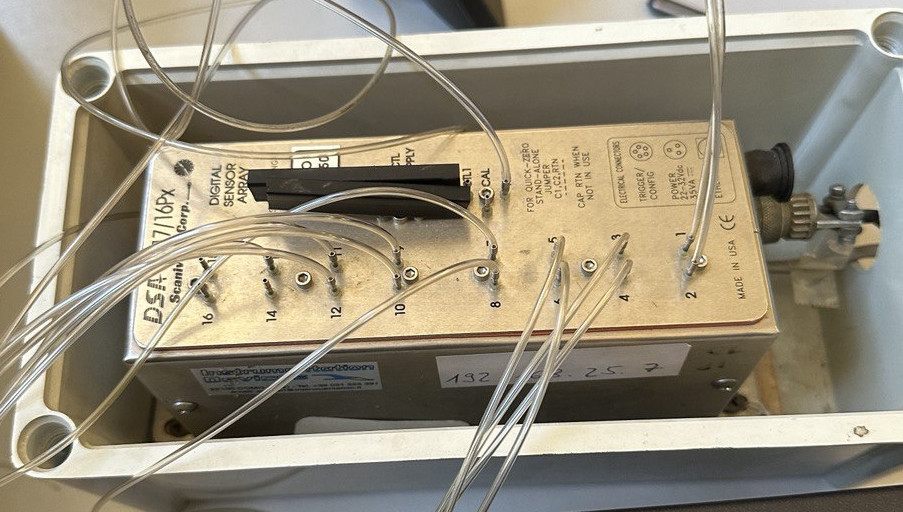
\includegraphics[width=.75\textwidth]{images/7/trasd.jpg}
    \caption{Trasduttore di pressione con i canali pneumatici collegati}
\end{figure}

\noindent Il trasduttore invia i dati attraverso un protocollo TCP/IP direttamente in Pascal ad un PC, che utilizza per la ricezione un software di acquisizione dati prioritario.\\\\
Pertanto, la catena di misura per la presente esercitazione è composta da:
\begin{itemize}
    \item Galleria del vento aperta con camera di prova a sezione rettangolare;
    \item Pannello di controllo per la regolazione della portata;
    \item 11 prese di pressione statica lungo il condotto;
    \item Una presa di pressione statica ed una presa di pressione totale per misurare la velocità del flusso sull'asse del condotto;
    \item Il trasduttore di pressione differenziale piezoresistivo DSA 3217;
    \item Il PC per l'elaborazione dati.
\end{itemize}

\newpage
\subsection{Procedura sperimentale}
Come prima cosa si misurano la pressione e la temperatura ambiente, dalle quali si ricava tramite la legge dei gas perfetti la densità e tramite la legge di Sutherland la viscosità dinamica:
\begin{equation*}
    \rho = \frac{p_{amb}}{RT_{amb}} \qquad \mu = 1.46\cdot10^{-6} \frac{T_{amb}^{3/2}}{T_{amb}+110} 
\end{equation*}
Successivamente si calcola il diametro idraulico del condotto, a partire dalla larghezza $B$ e dall'altezza $H$ del condotto:
\begin{equation*}
    D_{idr} = \frac{4A}{2P} = \frac{4BH}{2(B+H)} = 0.1135\ \text{m}
\end{equation*}
Utilizzando il pannello di controllo per la regolazione del numero di giri della ventola, si varia la portata e quindi il numero di Reynolds. Per ogni numero di Reynolds si acquisiscono i dati relativi alle prese di pressione in uscita dal trasduttore di pressione.\\\\
Ad ogni misura, il trasduttore registra una grande quantità di dati, ad una frequenza di campionamento di 20 Hz per un periodo di 60 secondi.\\\\
I dati grezzi mediati ottenuti per le quattro squadre sono riportati in appendice \ref{a7}.

\subsection{Analisi dati}
L'analisi dati per la presente attività è condotta con l'ausilio di un codice Python, riportato in appendice \ref{b7}.\\\\
Come primo passo si ricava il valore di pressione dinamica $q$ per ogni valore di portata:
\begin{equation*}
    q_{asse} = p_0 - p_s = \frac12 \rho U_{asse}^2
\end{equation*}
Poiché la velocità media nel condotto è circa uguale all'85\% della velocità sull'asse, si può calcolare la pressione dinamica media:
\begin{equation*}
    \overline q = (0.85)^2 q_{asse} 
\end{equation*}
Da cui deriva direttamente il valore di velocità media:
\begin{equation*}
    \overline U = \sqrt{\frac{2\overline q}\rho}
\end{equation*}
Quindi il numero di Reynolds:
\begin{equation*}
    Re = \frac{\rho \overline U D_{idr}}{\mu}
\end{equation*}
Diagrammando i valori di pressione rilevati dalle prese di pressione statica lungo il condotto, si ottiene un andamento linearmente decrescente:
\begin{figure}[H]
    \centering
    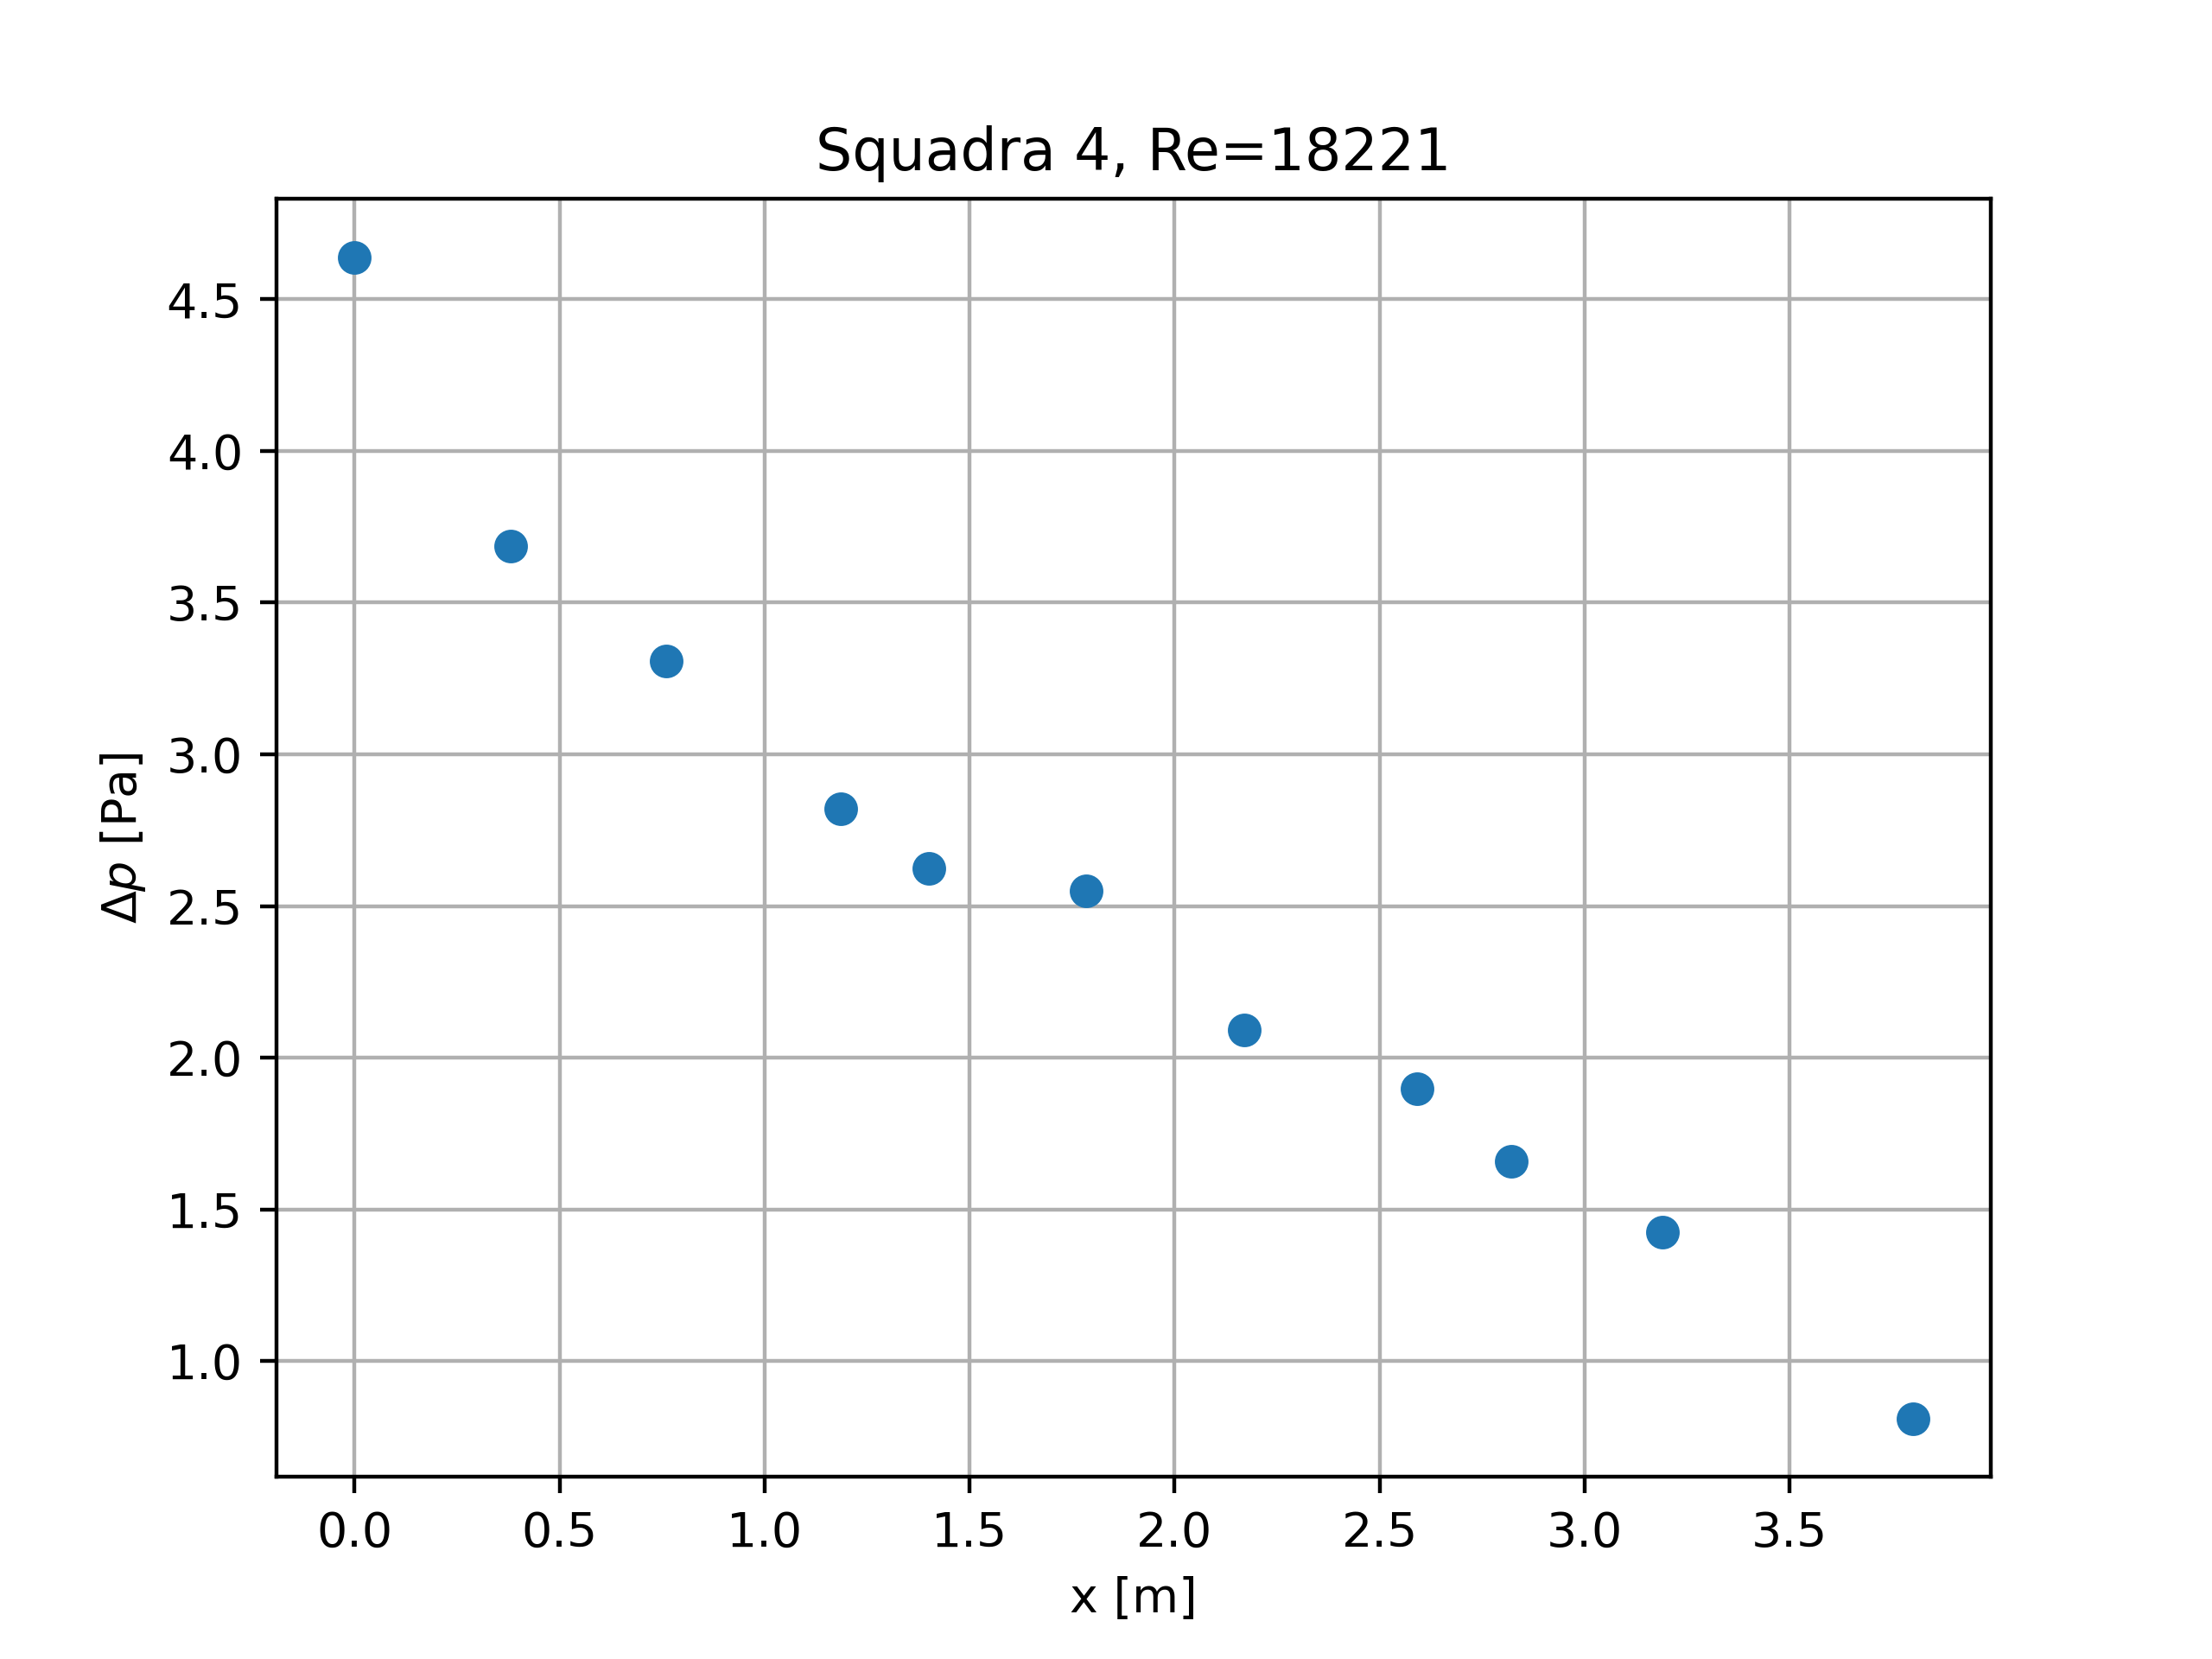
\includegraphics[width=.65\textwidth]{images/7/p.png}
    \caption{Esempio di variazione di pressione lungo il condotto}
\end{figure}

\noindent Pertanto, si può pensare di interpolare linearmente i dati ottenuti per ricavare il gradiente di pressione (negativo, perché la pressione diminuisce lungo il condotto). Si ricava quindi un valore di gradiente di pressione $dp/dx$ per ogni numero di Reynolds e si ottiene il seguente diagramma:
\begin{figure}[H]
    \centering
    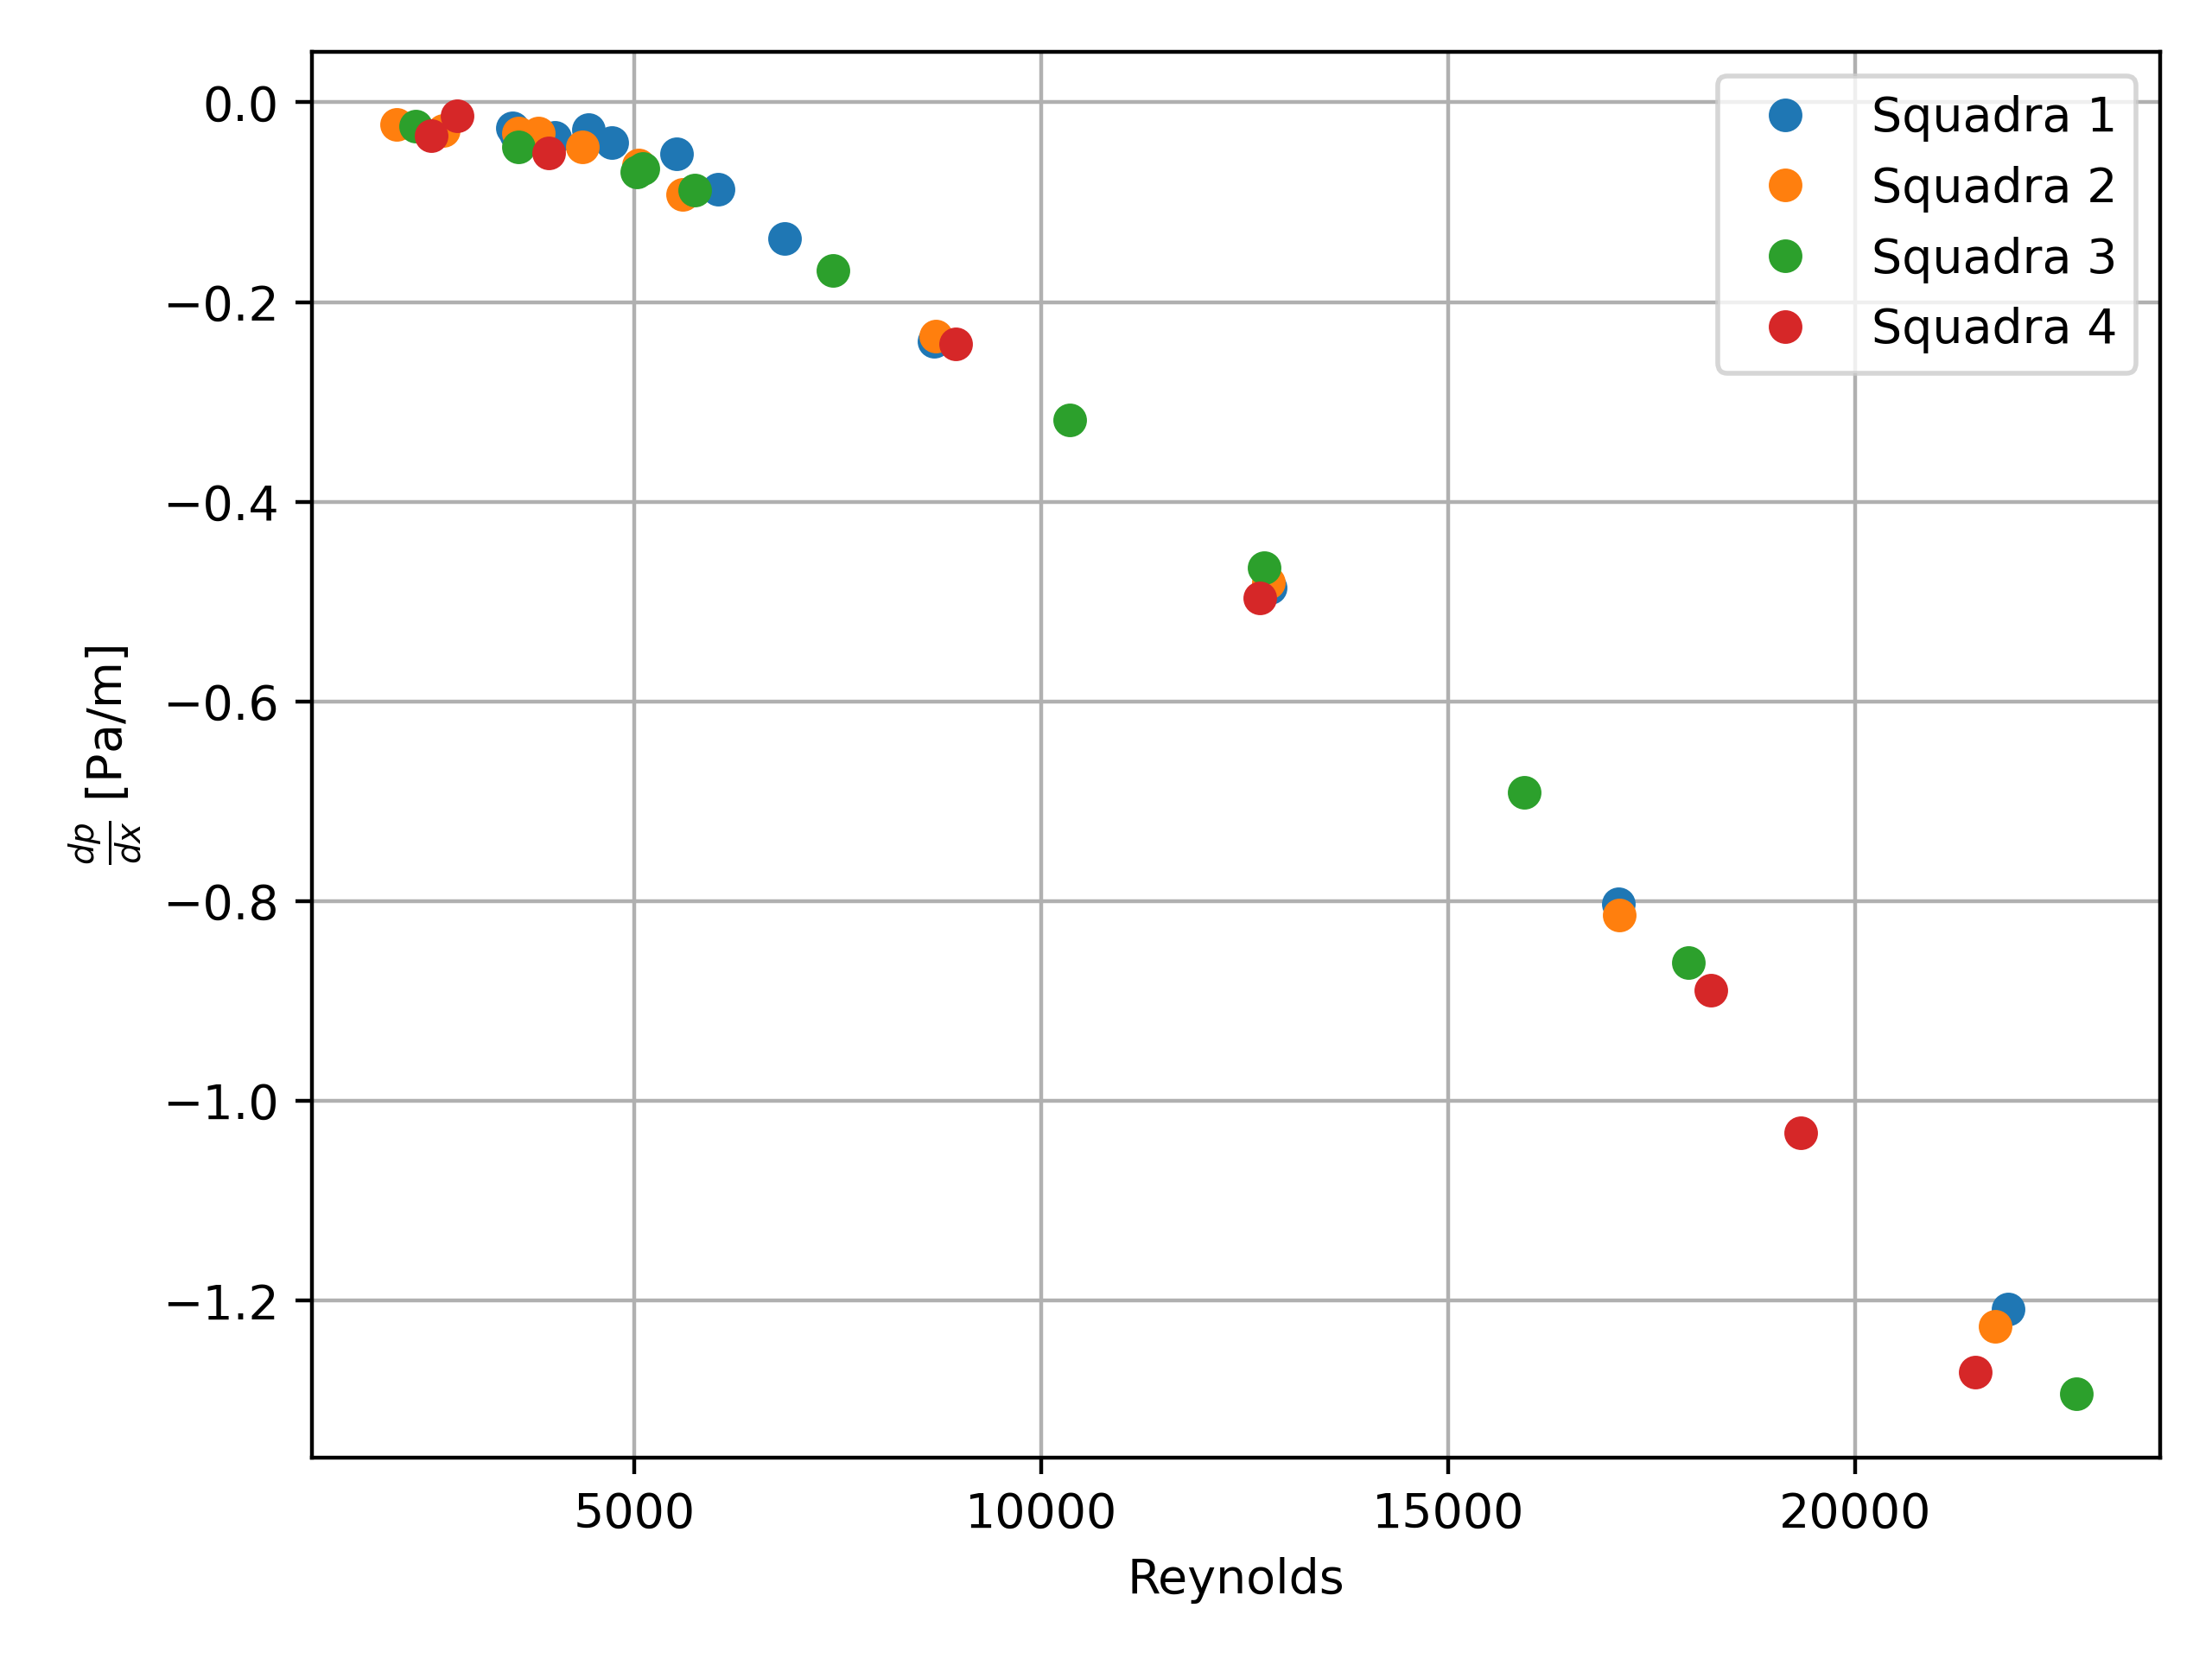
\includegraphics[width=.7\textwidth]{images/7/dpdx.png}
    \caption{Gradiente di pressione in funzione del numero di Reynolds}
\end{figure}

\noindent Si osserva come l'andamento del gradiente di pressione, per un certo valore di numero di Reynolds, cambia pendenza. Tale punto individua la transizione dal regime laminare al regime turbolento.\\\\
Si calcola infine il coefficiente di caduta di pressione $\lambda$:
\begin{equation*}
    \lambda = \frac{dp/dx}{\overline q/D_{idr}}
\end{equation*}
I risultati ottenuti sono confrontati con le seguenti leggi empiriche:
\begin{equation*}
    \begin{split}
        \text{Per } Re < Re_{cr} \quad &\Rightarrow \quad \lambda = \frac{64}{Re} \text{ per sezione circolare;}\\
        \text{Per } Re < Re_{cr} \quad &\Rightarrow \quad \lambda = \frac{96}{Re} \text{ per sezione rettangolare;}\\
        \text{Per } Re_{cr} < Re < 10^5 \quad &\Rightarrow \quad \lambda = \frac{0.32}{Re^{1/4}} \text{ bassa turbolenza;}\\
        \text{Per } 10^5 < Re < 10^8 \quad &\Rightarrow \quad \lambda = \frac{0.12}{Re^{1/6}} \text{ alta turbolenza.}
    \end{split}
\end{equation*}
Nel caso in esame, sono utili solo la seconda e la terza di queste leggi. Si ottiene quindi il seguente diagramma:
\begin{figure}[H]
    \centering
    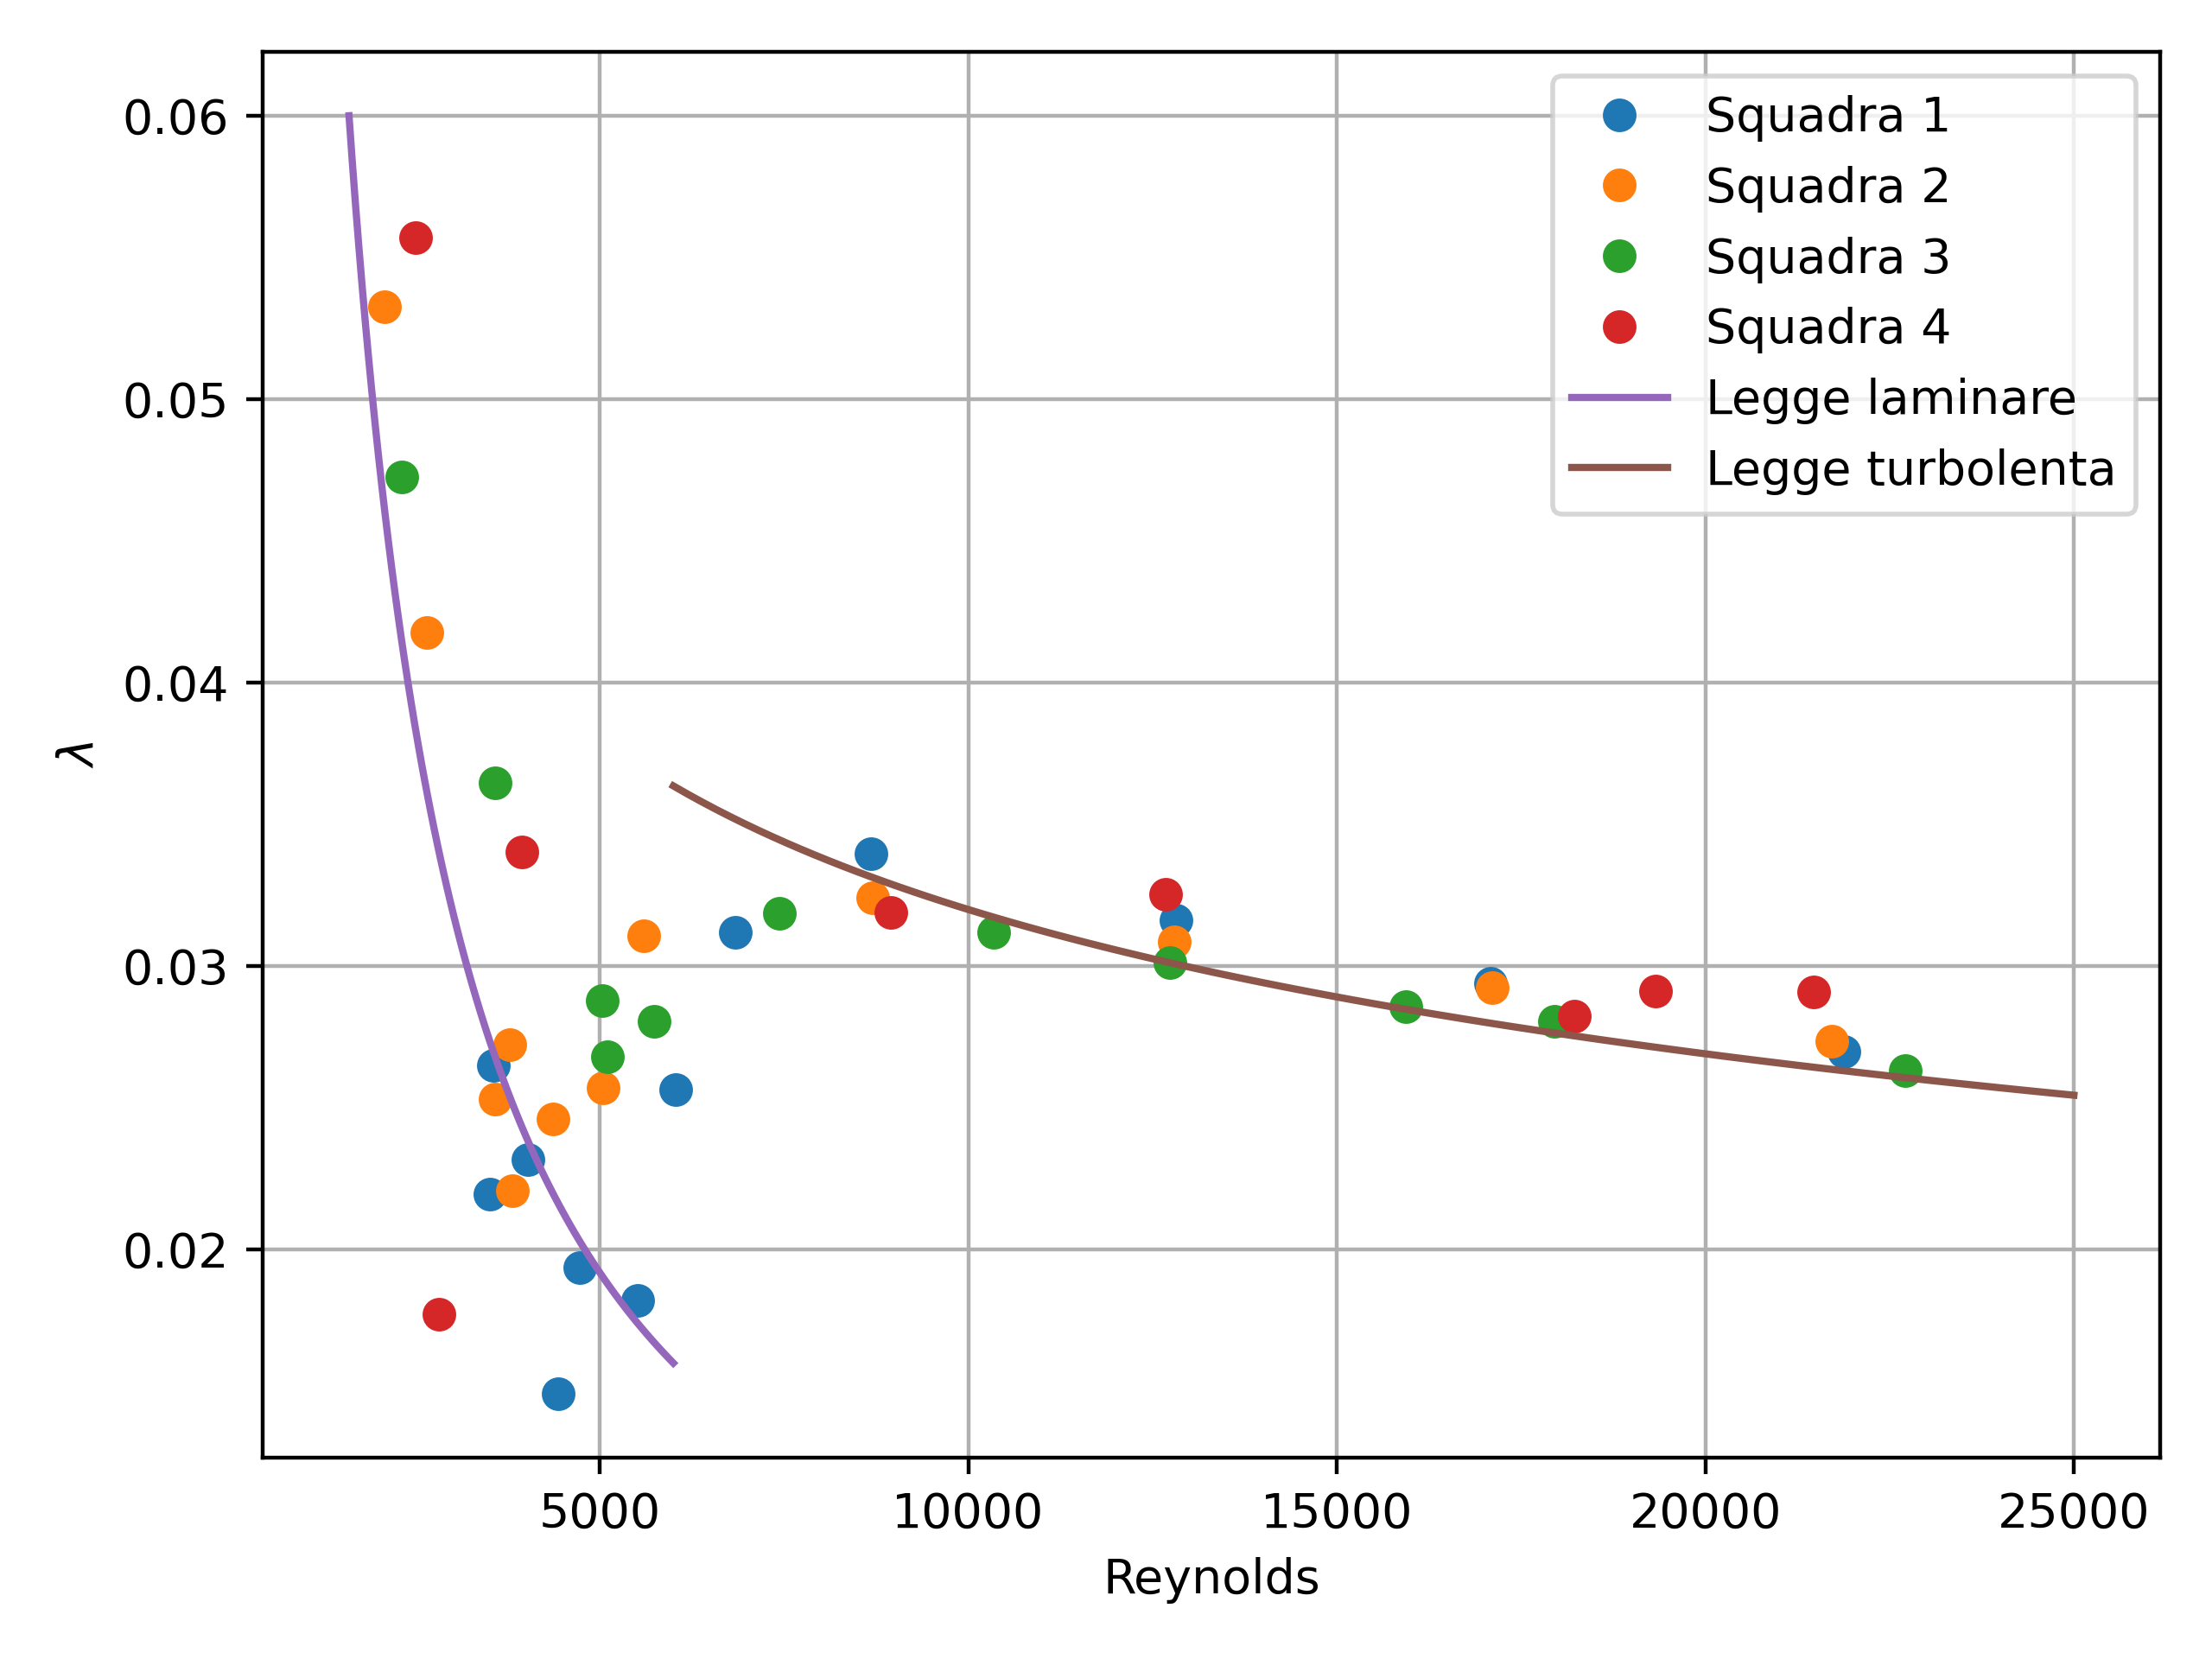
\includegraphics[width=.92\textwidth]{images/7/lambda.png}
    \caption{Coefficiente di caduta di pressione $\lambda$ in funzione del numero di Reynolds}
\end{figure}

\noindent Tale diagramma è solitamente espresso in scala logaritmica:
\begin{figure}[H]
    \centering
    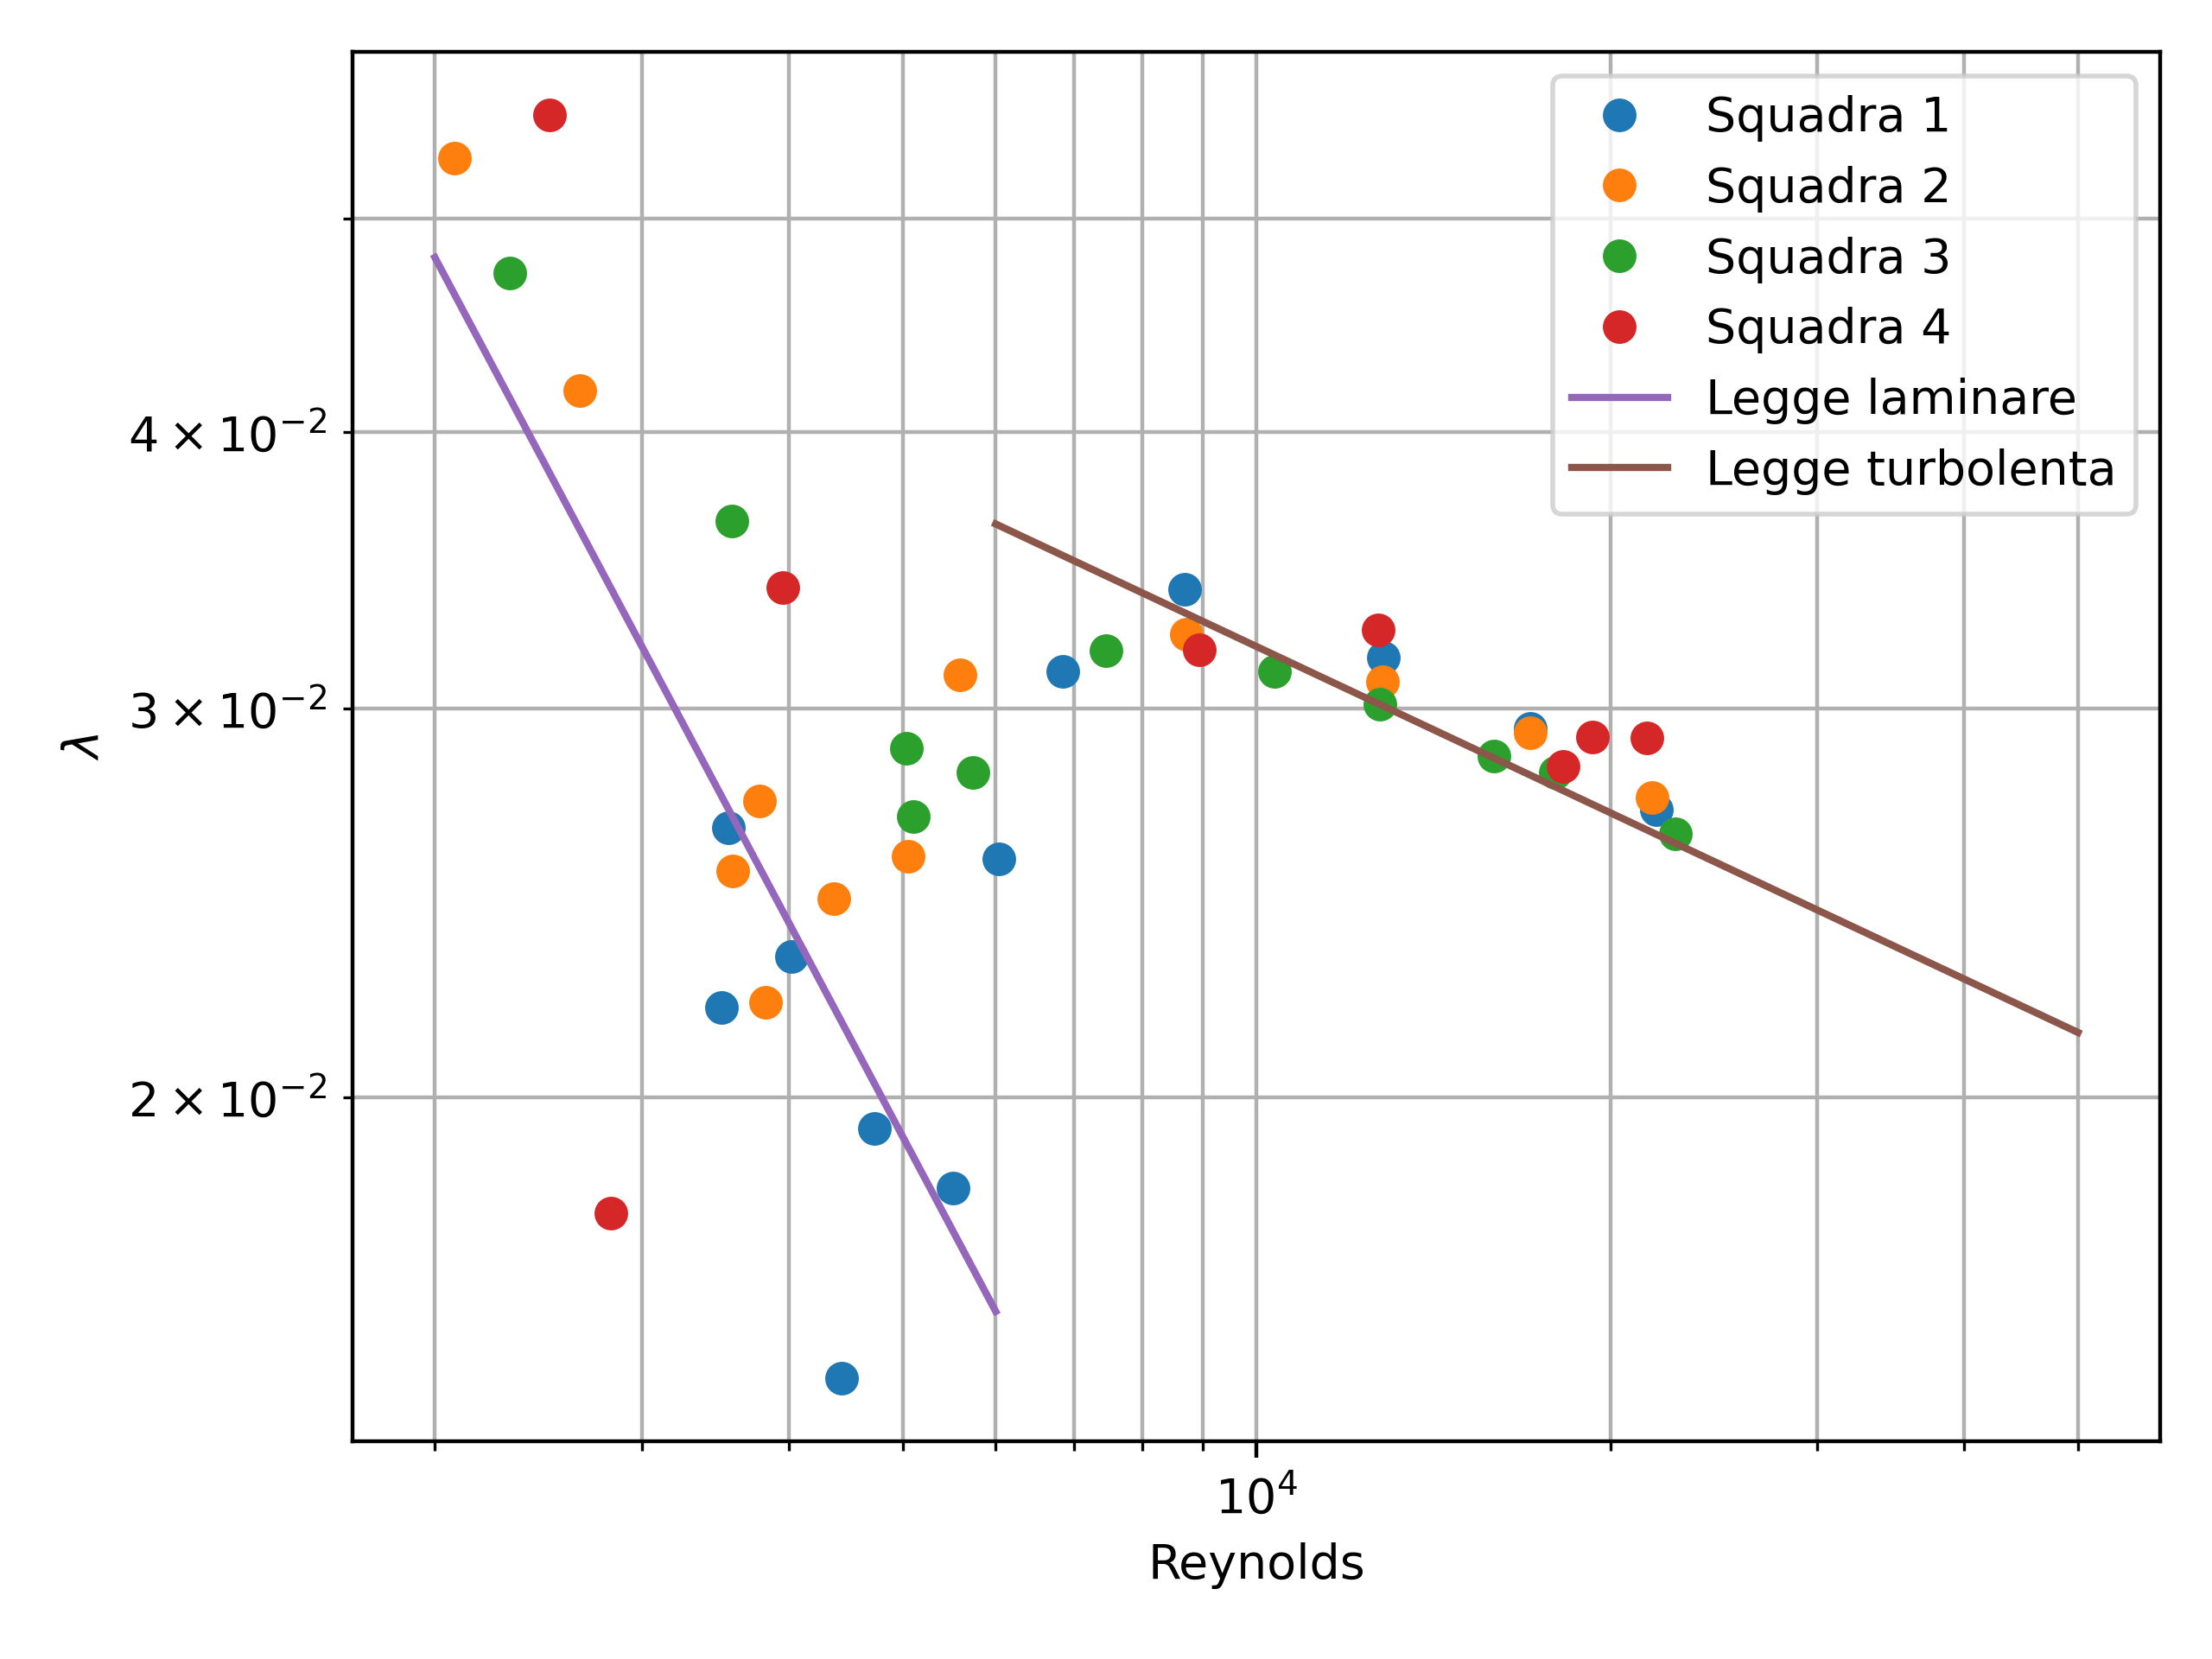
\includegraphics[width=.92\textwidth]{images/7/lambdaloglog.png}
    \caption{Coefficiente di caduta di pressione $\lambda$ in funzione del numero di Reynolds}
\end{figure}

\noindent Si osserva come i dati sperimentali ottenuti rispecchino affidabilmente le leggi teoriche-empiriche.\\\\
Dai diagrammi $\lambda(Re)$ riportati si può stimare un valore del numero di Reynolds critico, ovvero quel numero di Reynolds in cui avviene la transizione da laminare a turbolento, pari a circa $Re_{cr}\approx6000$. Come atteso, il numero di Reynolds critico per un condotto a sezione rettangolare è maggiore di quello per un condotto a sezione circolare ($Re_{cr,circ}\approx 2300$).